\documentclass[12pt, a4paper]{article}
\setlength{\headheight}{20pt}
%\renewcommand{\baselinestretch}{1.5}
\usepackage[margin=3cm]{geometry}
\usepackage{setspace}
\usepackage[english,danish]{babel}
%\onehalfspacing
\setstretch{1.2}
%\usepackage{mathptmx}% Times Roman font
%\usepackage{utopia}
%\usepackage{newcomputermodern}
\usepackage{lmodern}
\usepackage[colorlinks=true,linkcolor=black,anchorcolor=black,citecolor=black,filecolor=black,menucolor=black,runcolor=black,urlcolor=black]{hyperref}
\usepackage{varwidth}
\usepackage{amsmath}
\usepackage{amsthm}
\usepackage{xfrac}
\renewcommand\qedsymbol{$\blacksquare$}
\usepackage{amssymb}
\usepackage{mdframed}
\usepackage[T1]{fontenc}
\usepackage{fancyhdr}
\usepackage{pgfplots}
\usepackage{csquotes}
\usepackage{footnote}
\newcommand\s{30} %samples i grafer. set til 1000, 80 for arbejde
%\newcommand{\doubleunderline}{\underline{\underline{}}}
\usepackage{lipsum}
\usepackage{blindtext}
%flyta myndir
\usepackage{graphicx}
\usepackage{float}
\usepackage{sidecap}
%flyta myndir end
\fboxrule=1pt
\fboxsep=4pt
\usepackage{titlesec}
\titleformat{\section}
{\LARGE \bfseries}
{\thesection}
{1em}
{}

\titleformat{\subsection}
{\large \bfseries}
{\thesubsection}
{0.5em}
{}

%bruka inkscapefílir
\usepackage{import}
\usepackage{xifthen}
\usepackage{pdfpages}
\usepackage{transparent}

\newcommand{\incfig}[1]{%
    \def\svgwidth{6.00cm}
    \import{./figures/}{#1.pdf_tex}
}
%\renewcommand*\contentsname{Indholdsfortegnelse}
\renewcommand{\figurename}{Figur}
%bruka inkscapefílir end

\makeatletter
\patchcmd{\csq@bquote@i}{{#6}}{{\emph{#6}}}{}{}
\makeatother



%\usepackage[backend=biber,sorting=nty,style=verbose]{biblatex}
\usepackage[backend=biber,sorting=nty, style=authoryear-ibid]{biblatex}
\addbibresource{bibliografi.bib} %Imports bibliography file
\DeclarePrintbibliographyDefaults{heading=none}
\title{Taylorpolynomier}
%\author{Jákup H. Lützen}
\date{Februar 2022}
%\pagestyle{fancy}
%\fancyhead{}
%\fancyfoot{}
\AtBeginDocument{\let\textlabel\label}%
\begin{document}
\selectlanguage{danish}
\begin{refsection}
\begin{titlepage}
   \centering
    \vfill
%    \maketitle
    {\huge 
    Taylorpolynomier\\
    \vspace{0.5cm}
    \large
    SSO - Matematik A\\
    \vspace{0.25cm}
    Jákup Lützen - Februar 2022
    }    
    \vfill
%    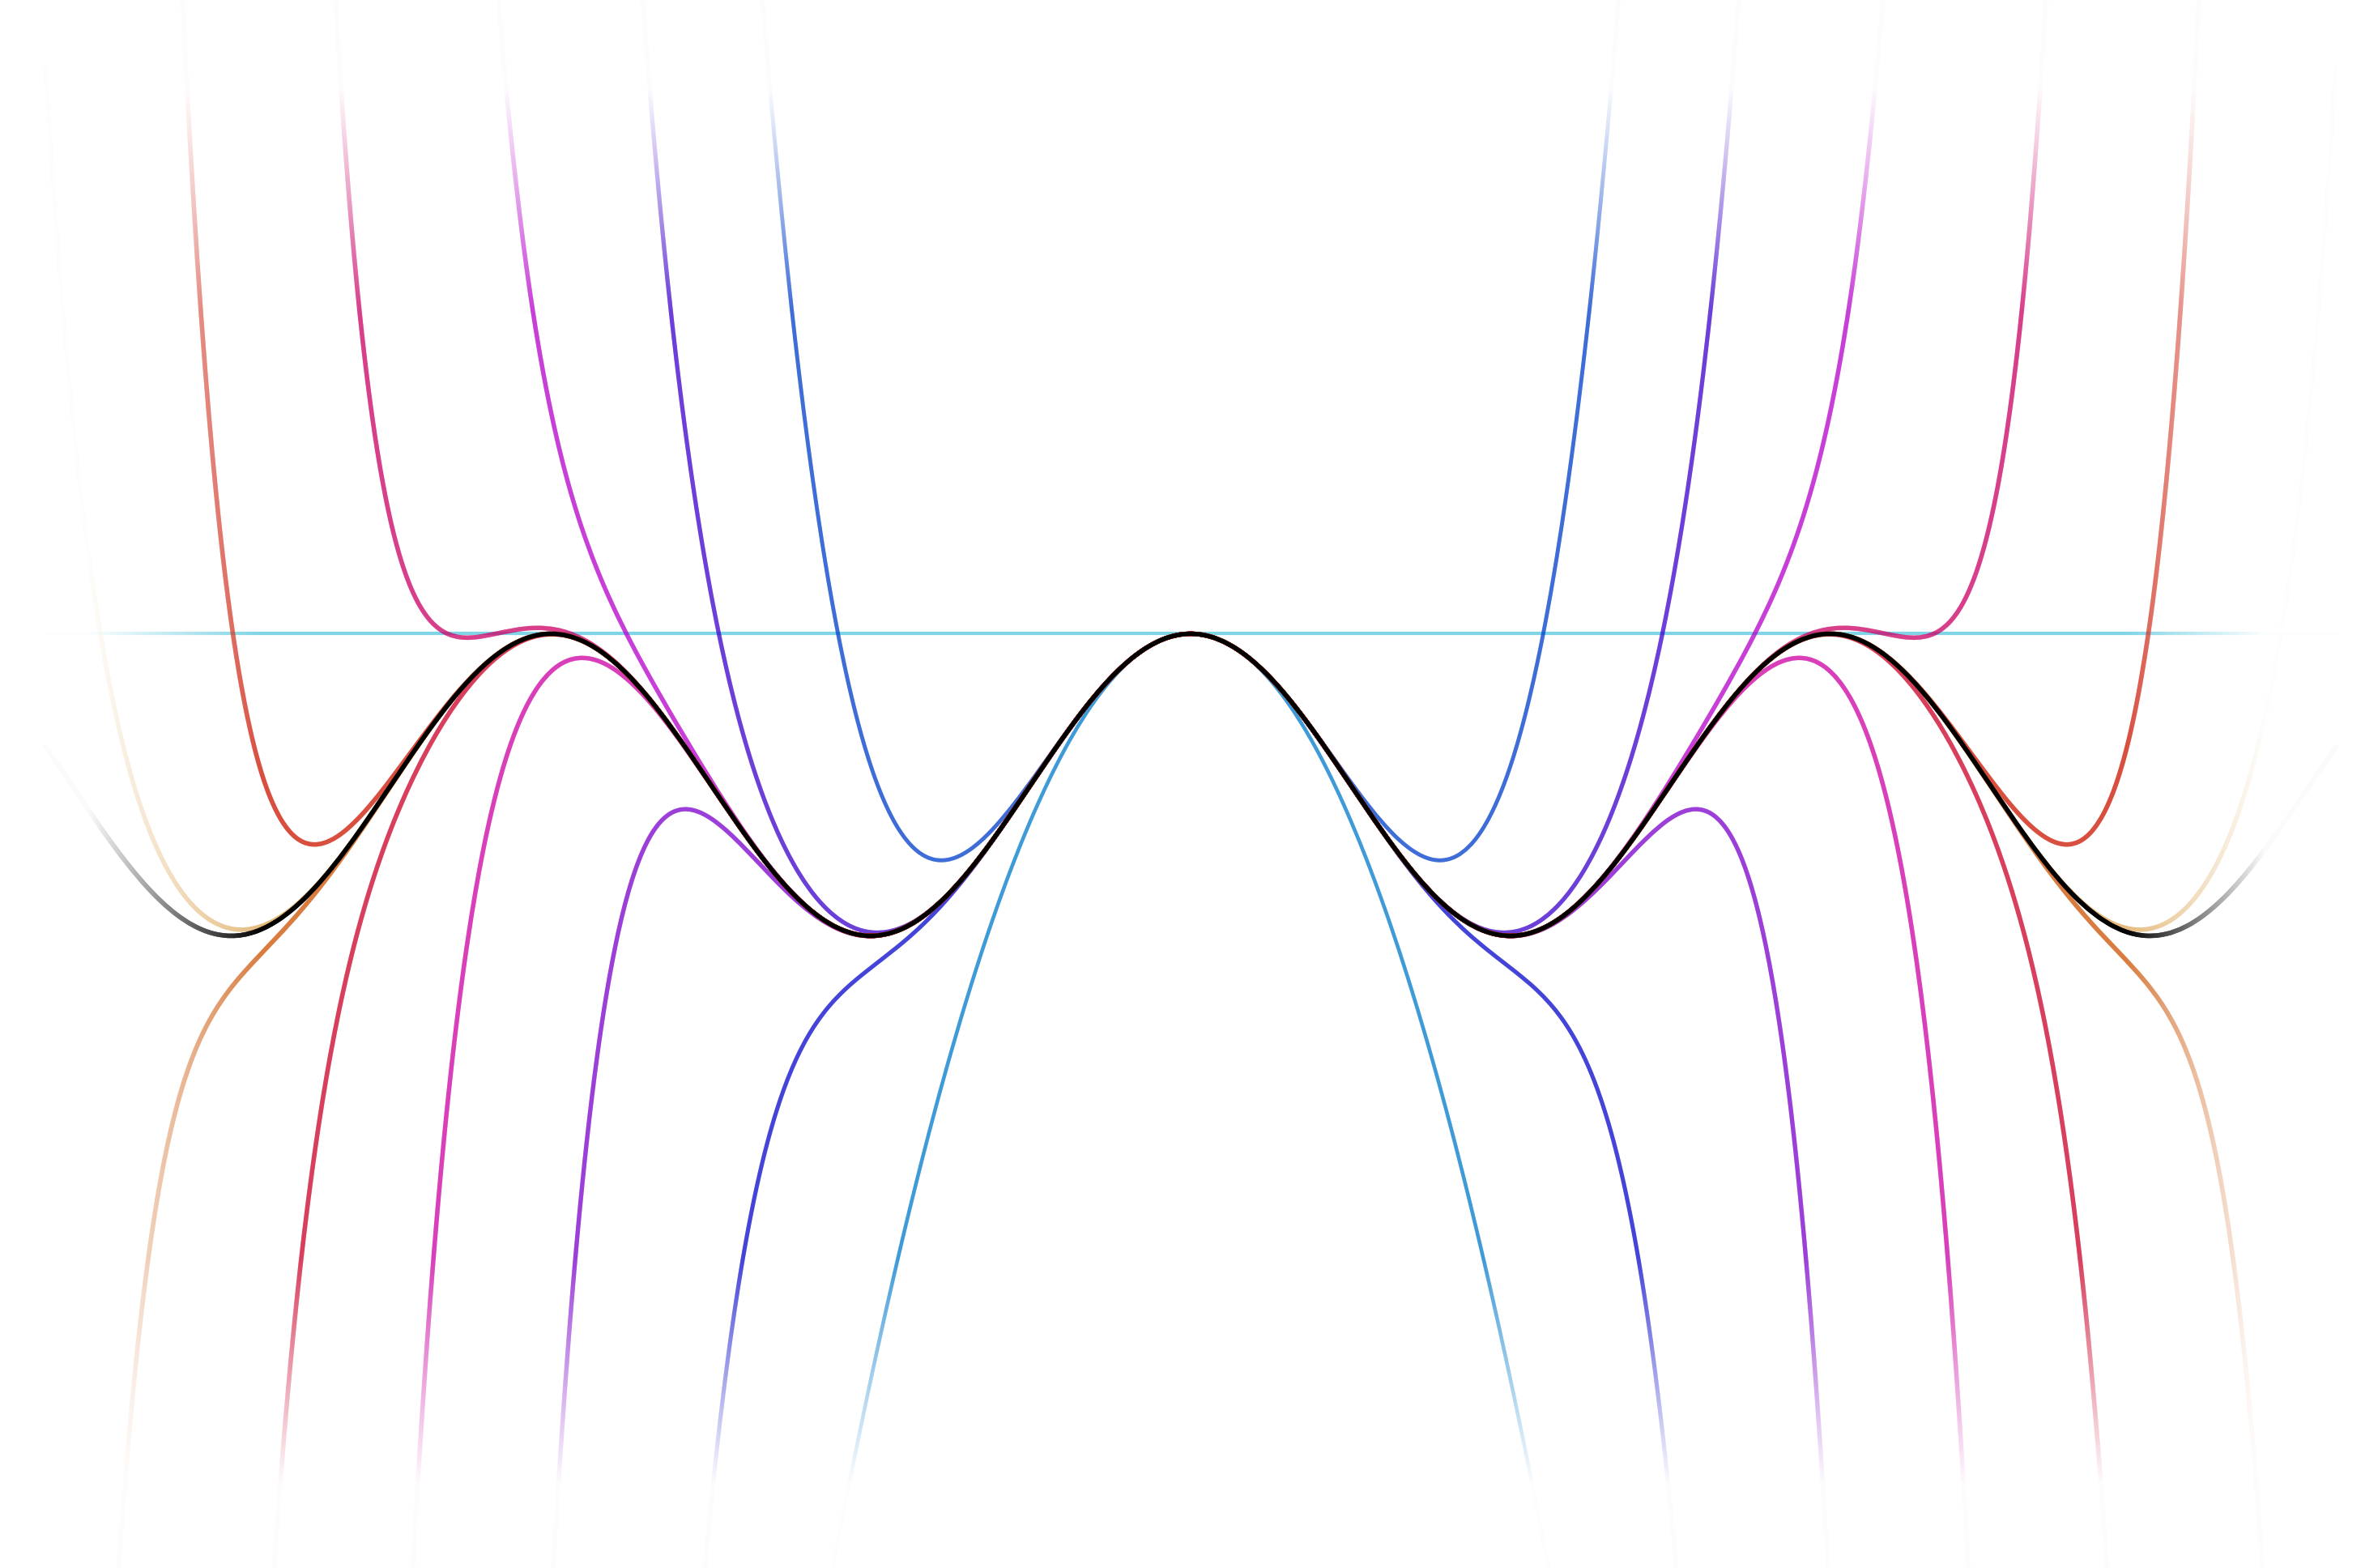
\includegraphics[width=\textwidth]{figures/forside3edit2.png} % also works with logo.pdf
   
    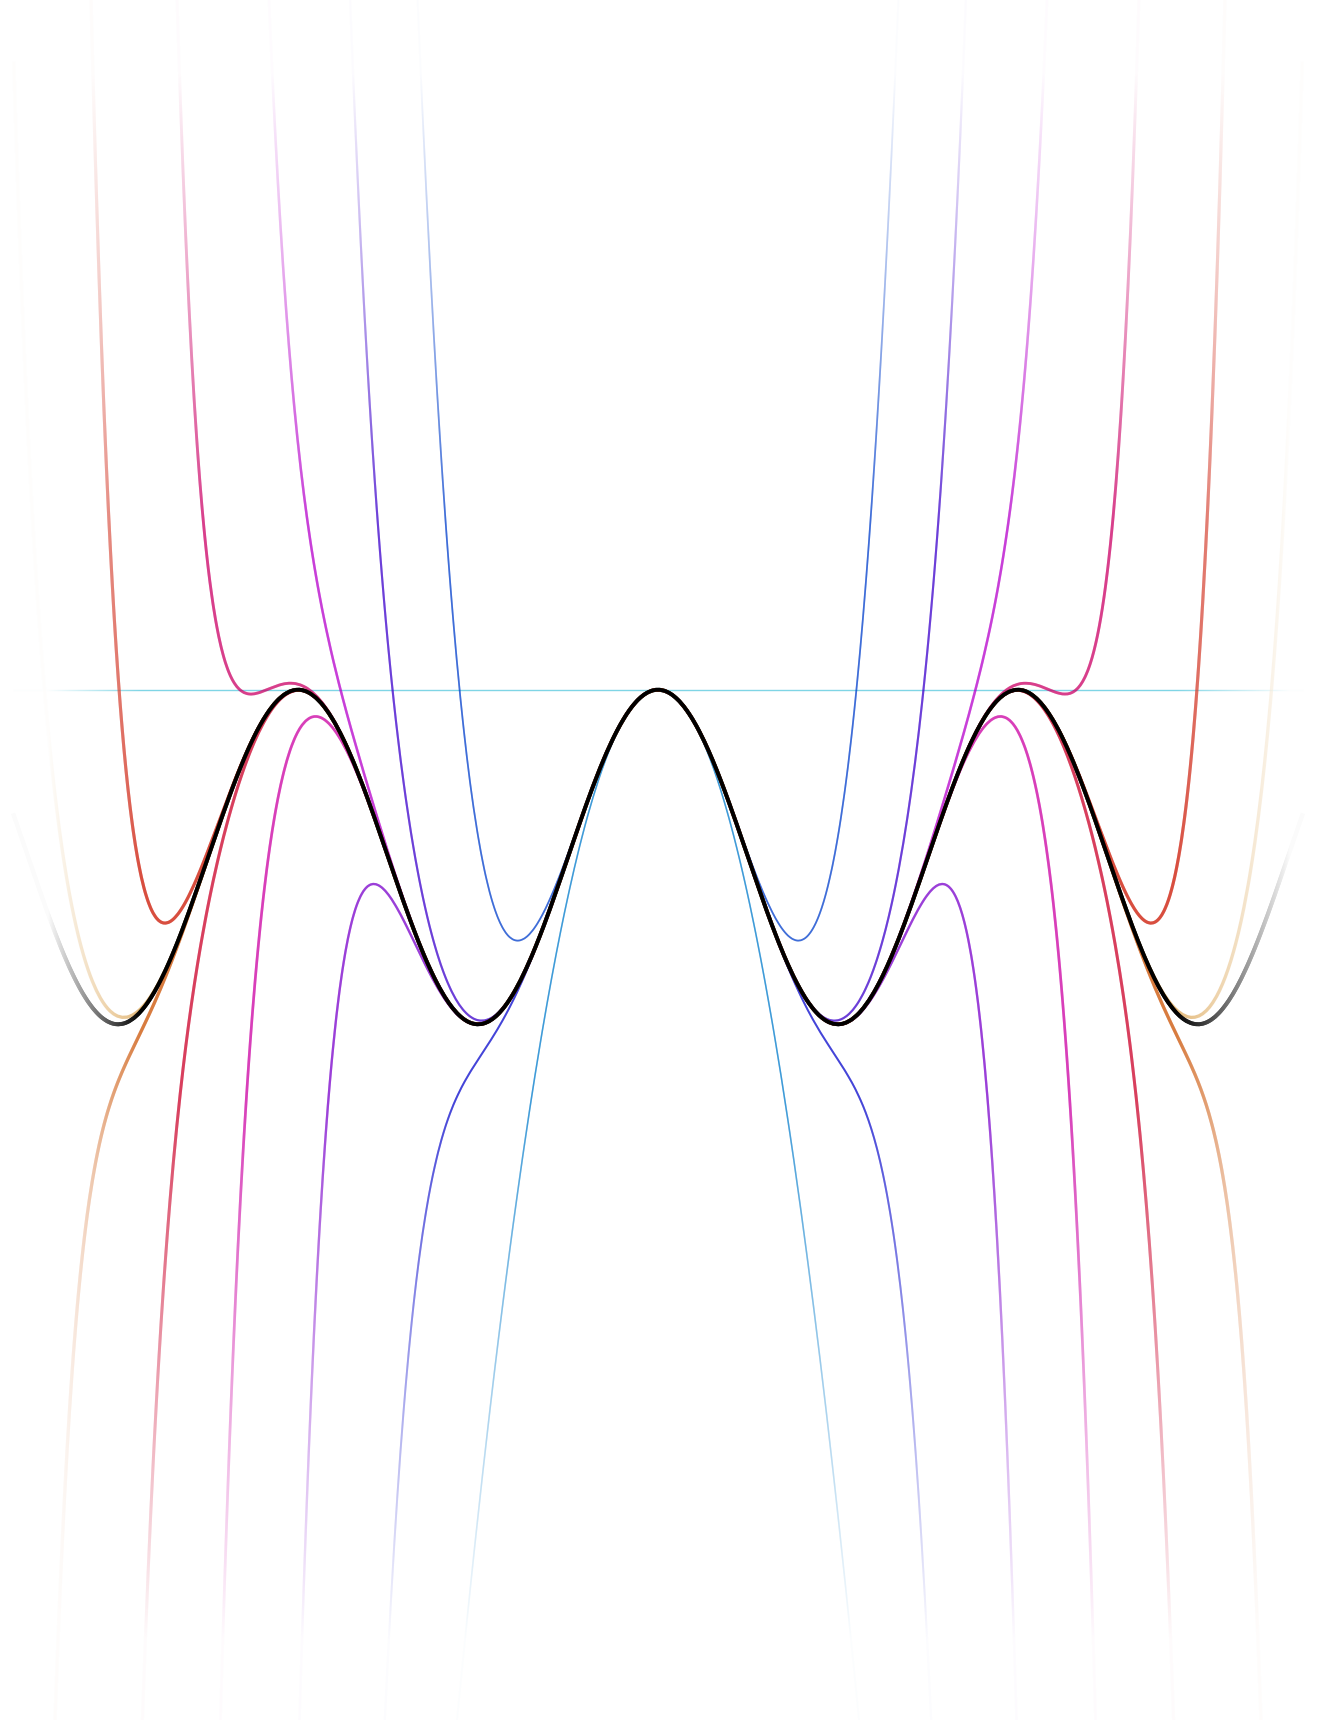
\includegraphics[width=\textwidth]{figures/forside4edit.png} % also works with logo.pdf
    \vfill
    \vfill
\thispagestyle{empty}

\end{titlepage}
%%%%% \footnote{hey} fyri vanligan footnote
%%%%%\footcite{talogrækker} fyri referencu
%%%%% :set spell spelllang=da (fyri at byrja spellcheck)
%%%% :set nospell fyri at sløkkja
%\setcounter{page}{2} % Set dette hvis første side tæller med i sidecount 
\section*{Resume} %150 ord (det essentielle i min opgave, dvs ca 8 linjer
\blindtext[1-2]
\tableofcontents
\newpage



\section{Indledning} %ca en halv side til en side. I egne ord, hvorfor dette er interessant. God ide at slutte af med problemformuleringen, "Og her vil jeg..."
Matematik kan til tider synes firkantet og rigidt, hvor abstrakte forhold opskrives i eksakte formler, og hvor der ikke er plads til kreativitet. 
Dykker man dybere ind i faget vil man dog opdage, at dette ikke er tilfældet, og at der er mange situationer, hvor man gør kreativt brug af relativt ueksakte værktøjer. Et af disse er såkaldte Taylorpolynomier.


I matematikkens verden findes der alverdens slags funktioner, hvor nogle er mere medgørlige end andre. Nutidens computerteknik kræver desuden hurtig og praktisk behandling af alle disse formler, og i den forbindelse indtræder Taylorpolynomier ofte.\\
\\
Taylorpolynomier er ingen ny opfindelse. De dukkede for første gang op i 17-18. århundrede, men hvordan blev de opdaget? Der er ingen tvivl om at de har haft stor indflydelse på måden som matematik bliver behandlet i dag, men hvordan ved man om de er korrekte, i hvilken grad ved man det, og hvorfor er det i det hele taget relevant i dag?\\
\\
Denne opgave vil beskrive den historiske baggrund for Taylorrækken, bevise formlen for Taylorrækken, undersøge dens restled, samt undersøge hvilke praktiske anvendelser Taylorpolynomier har i dag.

\section{Taylorrækkens historie} % Redegørelse Egne ord. Ikke inddrage citater (fordi så bliver det analyserende).
Matematikeren Brook Taylor (1685 - 1731) er navnefader til hvad vi i dag kalder Taylorpolynomier, efter at han i 1715 offentliggjorde en generel formel, der for samtidens matematikere var kendt som Proposition 7, Corollary 2 fra hans \textit{Methodus}.
Taylors formel ser således ud i sin moderne form:\footcite[s. 247]{roy_2021}$^,$\footcite[s. 72]{feigenbaum_exact_sciences}
\begin{equation*}
   f(x)=f(x_0)+f(x-x_0)\frac{f'(x_0)}{1!}+(x-x_0)^2\frac{f''(x_0)}{2!}+\cdots. 
\end{equation*}
Dette kan naturligvis også skrives som:
\begin{equation*}
    f(x)=\sum_{n=0}^{\infty}\frac{f^{(n)}(x_0)}{n!}(x-x_0)^n.
\end{equation*}
Men Taylor var dog ikke den første der tænkte disse tanker. Man ved i dag, at der var mindst fem andre forløbere: James Gregory, Newton, Leibniz, Johann I. Bernoulli, og Abraham De Movre.\footcite{feigenbaum_exact_sciences}
\subsection{Newton, Gregory og Bernoulli}

Taylorpolynomier bygger på en indseelse, at der er en forbindelse mellem en funktions koefficienter og dens afledte. Denne indseelse viser Isaac Newton (1643 - 1727) for første gang i hans \textit{Principia} (1687), og få år senere giver han et egentligt eksempel af Taylors formel i sin \textit{De Quadratura Curvarum} (1691 - 92), som han aldrig færdiggjorde. Dele af denne tekst blev udgivet med titlen \textit{Tractatus de Quadratura Curvarum}, men Taylors formel blev desværre udladt.\footcite[s. 248]{roy_2021} Newton havde altså opdaget disse samme principper femogtyve år tidligere end Taylor, uden at de blev udgivet.\\
\\
Newton havde i det hele taget svært ved at udgive sine findelser før han blev kendt i videre kredse, hvilket til tider voldte ham problemer i at blive anerkendt for sine opdageser. \footcite[s. 116]{uendeligerækker}\\
En af konsekvenserne af dette var den kendte kontroversi imellem Newton og Gottfried Wilhelb Leibniz (1646 - 1716), da de ifølge Mejlbo:
\blockquote{blev indviklede i en ulykkelig strid om ophavsretten til differential- og integralregningen. Den gik værst  ud over Leibniz. Royal Society dømte ham - ganske uberettiget - for plagiat}.\footcite[s. 103]{uendeligerækker}\\
En af Leibnitz' største fortalere i denne prioritetsstrid var Johann Bernoulli (1667 - 1748), som i slutningen af 1690'erne også havde udgivet en formel der lignede Taylors formel. Mejlbo skriver om Bernoulli at: \blockquote{\dots han havde et voldsomt temperament, så han overfusede Taylor med beskyldninger for plagiat.}\footcite[s. 111]{uendeligerækker}. \textcolor{red}{mere om Bernoulli og Taylors rivalisering}\\
\\
Den tidligste opdager af Taylors formel var dog nok den Skotske matematiker James Gregory (1638 – 1675).\\
\textcolor{red}{\textbf{Mere om Gregory}} 
\newpage
\section{Analyse} % Kød og kartofler. Brug modellen (introducere citatet, så kommer citatet, og så kommenterer man.
\subsection{Pædagogisk gennemgang (\textcolor{red}{arbejdstitel})}
Man kan opnå en simpel intuitiv forståelse for Taylorpolynomier med følgende fremgangsmåde:\\
Man ønsker at approksimere en given funktion $f(x)$ fra x-værdien $x_0$. I dette eksempel bruges funktionen $f(x)=e^x$, og $x_0=1$.\\
\begin{figure}[h!]
     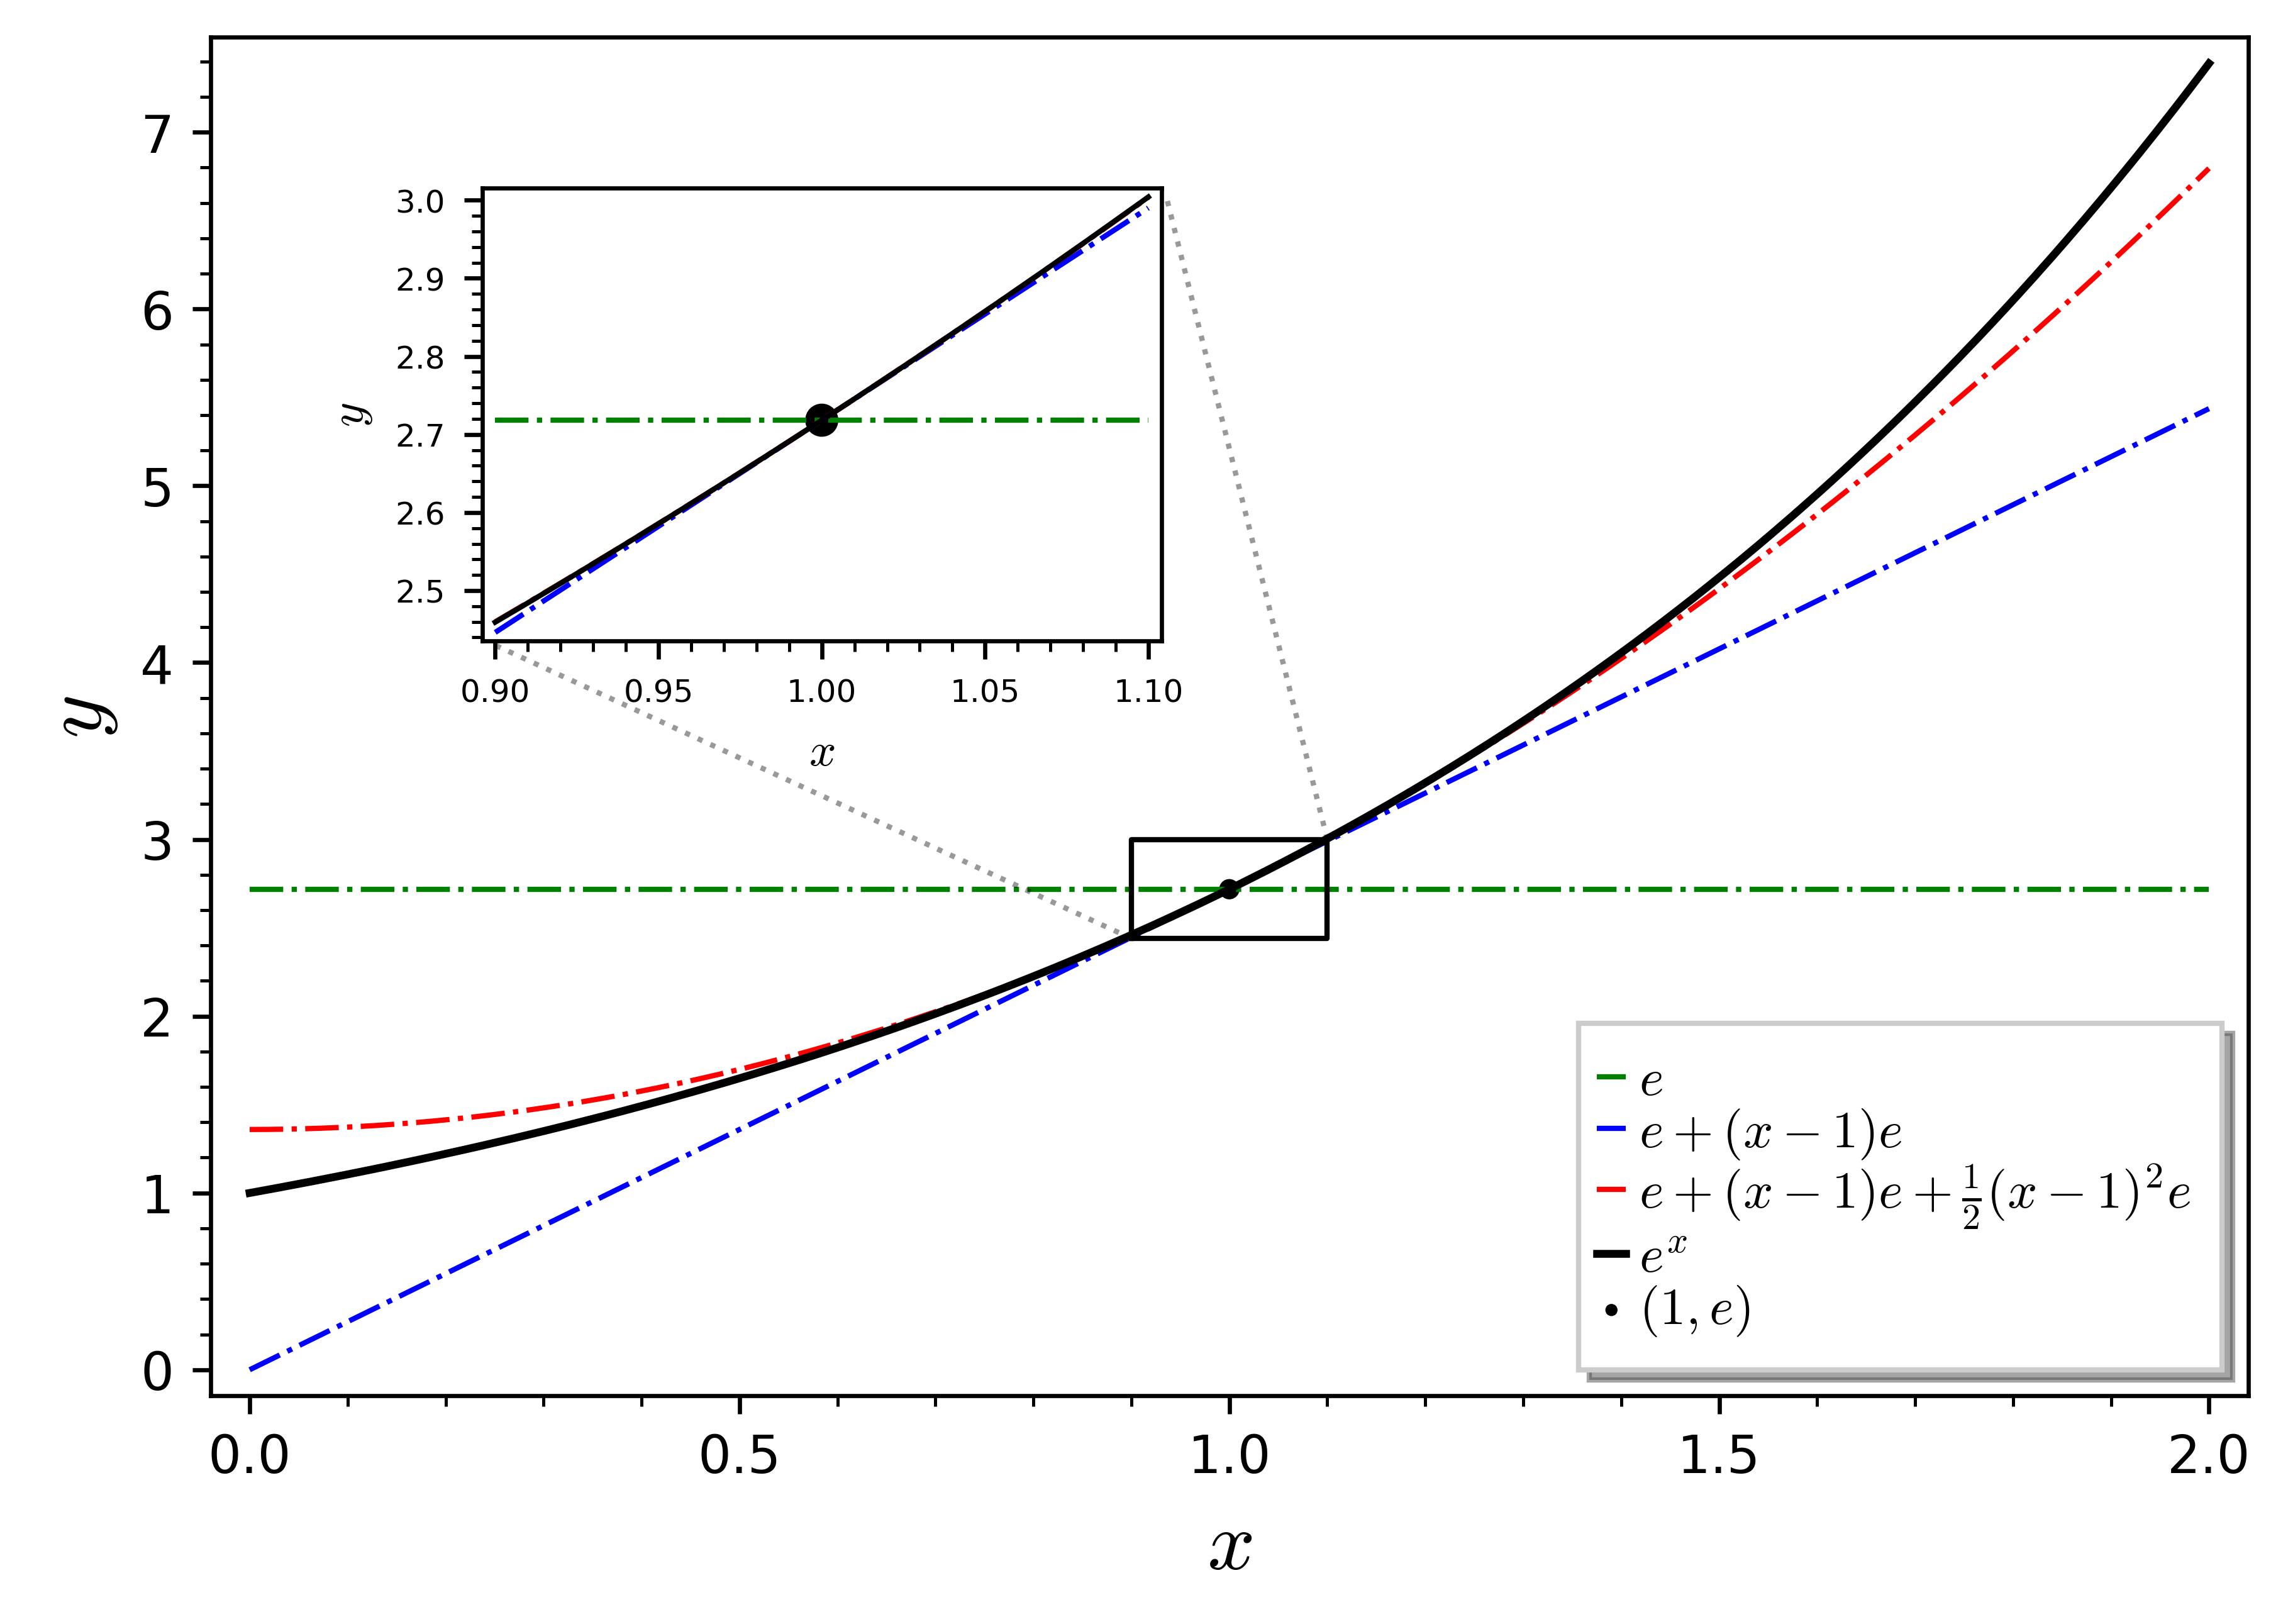
\includegraphics[width=\textwidth]{figures/ex-eksempel.png}
     \caption{Nulte- første- og andengrads Taylorpolynomium for $e^x$}
     \label{fig:ex-012tpol}
\end{figure}\\
Den simpleste approksimation kunne være en konstant funktion, som deler værdi med $f(x)$ på $x_0$ (\textit{Figur \ref{fig:ex-012tpol}, grøn}).
\[
f(1)=e
.\] 
Dette er funktionens nultegrads Taylorpolynomium, som er en meget grov approksimation, da den er konstant. Den kan dog forbedres ved at tilføje den korrekte hældning på punktet. Dette genkendes som ligningen for tangenten til grafen for $f$ i $P\big(x_0,f(x_0)\big)$.\footcite[s. 24, frml. 130]{formelsamling}
\[
\begin{aligned}
    y&=f'(x_0) \cdot (x-x_0)+f(x_0)\\
    \Updownarrow\quad &=f(x_0)+f'(x_0) \cdot (x-x_0)
\end{aligned}
.\] 
Den gældende funktion indsættes, og hermed findes funktionens førstegrads Taylorpolynomium  (\textit{Figur 1, blå}).\\
\[
\begin{aligned}
    y&=e+e\cdot (x-1)
\end{aligned}
.\] 
Nu er værdien samt hældningen på $x_0$ korrekt. Dette er ikke en dårlig approksimation for værdier tæt på $x_0$ (se Figur 1.) For at forbedre approksimationen kan man tilføje den korrekte krumning. 
\subsection{Bevis for Taylorpolynomiet}
\begin{proof}[Bevis]
    
Vi har indtil videre set, hvordan en tangent og en parabel blev brugt som en polynomisk approksimation for en funktion $f(x)$. Vi kan generalisere denne approksimationsmetode tæt på $x=x_0$ med et  $n$-tegrads polynomium.\\
\[
P_n(x)=c_0+c_1x+c_2x^2+ \cdots +c_nx^n
\] 
således at polynomiets værdi på $x_0$ stemmer overens med  $f(x_0)$. Det samme skal gælde for alle afledte, op til $n$ gange afledte funktioner, dvs:
 \begin{equation}\label{deafledtestemmer}
     \begin{aligned}
         P_n(x_0)&=f(x_0),\\
         P'_n(x_0)&=f'(x_0),\\
         P''_n(x_0)&=f'(x_0),\\
                   &\vdots\\
         P^{(n)}_n(x_0)&=f^{(n)}(x_0).
     \end{aligned}
\end{equation}
Eftersom det er $x_0$ vi har interesse i, giver det mening at udtrykke  $P_n$ på formen:
\begin{equation}\label{nybevis1}
   P_n(x)=c_0+c_1(x-x_0)+c_2(x-x_0)^2+\cdots+c_n(x-x_0)^n 
\end{equation}
For at finde konstanterne $c_0, c_1 \cdots c_n$ på punktet $x_0$, kan vi ganske enkelt indsætte $x=x_0$ i $P_n(x), P'_n(x) \cdots P^{(n)}_n(x)$. Vi bruger desuden ligning (\ref{deafledtestemmer}) at forbinde konstanterne med $f(x_0)$\\
%Når dette sættes ind i ligning (\ref{deafledtestemmer}), giver det:
Den første konstant er åbenlys, når vi indsætter $x=x_0$ i ligning (\ref{nybevis1})
 \begin{equation*}
    c_0=P_n(x_0)=f(x_0)
\end{equation*}
Derefter observerer vi den afledte funktion: 
\begin{equation}\label{førsteafledte}
        P'_n(x)=c_1+2c_2(x-x_0)+3c_3(x-x_0)^2+\cdots+nc_n(x-x_0)^{n-1}\\
\end{equation}
Vi kan nu på samme måde indsætte $x=x_0$ i ligning (\ref{førsteafledte}), og igen jævnføre med ligning (\ref{deafledtestemmer}), for at konkludere at:
\begin{equation*}
    c_1=P'_n(x_0)=f'(x_0)
\end{equation*}
Vi fortsætter samme fremgangsmåde, og observerer nu $P''_n(x)$.
\begin{equation}\label{andenafledte}
    P''_n(x)=2c_2+ 3\cdot2c_3(x-x_0)+\cdots+n(n-1)c_n(x-x_0)^{n-2}
\end{equation}
Når vi indsætter $x=x_0$ i ligning (\ref{andenafledte}) sær vi at $2c_2 = P''_n(x_0)=f''(x_0)$, hvilket betyder at:
\begin{equation*}
    c_2=\frac{1}{2}f''(x_0).
\end{equation*}
Nu begynder et mønster at vise sig. Eftersom de næste konstanter findes med gentagen differentiering af voksende potenser, vil konstanterne følge mønstret: 
\begin{equation*}
    \begin{array}{c c c}
        3\cdot2\cdot1\cdot c_3=f'''(x_0),\quad &4\cdot3\cdot2\cdot1\cdot c_4=f^{(4)}(x_0),\quad&5\cdot4\cdot3\cdot2\cdot1\cdot c_5=f^{(5)}(x_0)\\
        \Updownarrow&\Updownarrow&\Updownarrow\\
        c_3=\frac{f'''(x_0)}{3!},&c_4=\frac{f^{(4)}(x_0)}{4!},&c_5=\frac{f^{(5)}(x_0)}{5!}.
    \end{array}
\end{equation*}
Generelt, når vi indsætter $x=x_0$ i $P_n^{(k)}(x)$ ser vi at:
\begin{equation*}
    k!c_k=P_n^{(k)}(x_0)=f^{(k)}(x_0)
\end{equation*}
og derfor:
\begin{equation}\label{konstantergenerelt}
    \boxed{c_k=\frac{f^{(k)}(x_0)}{k!}}
\end{equation}
for $k=1,2,3,\cdots,n$. når vi husker at $0!=1$, og at den nulte afledte  $g^{(0)}$ af en funktion $g$ blot er selve funktionen $g$, indser vi at ligning (\ref{konstantergenerelt}) også gælder for $k=0$.\\
Dette giver os følgende sætning:\\
\\
   \begin{savenotes}
\begin{mdframed}
Antag at $f(x)$ er $n$ gange differentiabel på $x=x_0$. Lad $P_n(x)$ være $n$-tegrads polynomiet
\begin{equation}\label{taylorpolynomier}
    \begin{aligned}
        P_n(x)&=\sum_{k=0}^n\frac{f^{(k)}(x_0)}{k!}(x-x_0)^k\\
              &=f(x_0)+f'(x_0)(x-x_0)+\frac{f''(x_0)}{2!}(x-x_0)^2+\cdots+\frac{f^{(n)}(x_0)}{n!}(x-x_0)^n.
    \end{aligned}
\end{equation}
\renewcommand{\thempfootnote}{\arabic{footnote}} 
Så vil værdierne af $P_n(x)$ og dets første $n$ afledte funktioner stemme overens med $f(x)$ og dets første $n$ afledte funktioner på punktet $x=x_0$.\stepcounter{footnote}\footcite[s. 647-648]{calculuswithanalyticgeometry}$^,$\stepcounter{footnote}\footcite[s.1-2]{alsholm2}%det er nødvendigt at lave stepcounter før hver fodnote i mdframe, for at manuelt enumerate fodnote, når der er flere fodnoter i boksen
\end{mdframed}
   \end{savenotes} 
\end{proof}
\subsection{Taylorpolynomiers restled}
Når man approksimerer et funktion med dens Taylorpolynomium vil der altid opstå en fejl (udenfor udviklingspunktet $x_0$).\footcite[s. 4]{alsholm1}Til dette har man Taylors formel.\\
Taylors formel giver os muligheden for at approksimere fejlen, og derved vurdere hvilken grad Taylorpolynomiet skal føres til, for at fejlen holder sig indenfor en vis margin. Den giver os også mulighed for at endelig sætte lighedstegn funktionen og Taylors formel, dog med en ekstra ubekendt ($\xi$).\\
Tætheden som polynomiet $P_n(x)$ approksimerer funktionen $f(x)$ med, måles med differencen:\footcite[s. 650]{calculuswithanalyticgeometry}
\begin{equation}\label{restled}
    \begin{aligned}
        R_n(x)&=f(x)-P_n(x),\\
        \Leftrightarrow \quad f(x)&=P_n(x)+R_n(x).
    \end{aligned}
\end{equation}
\subsection{Bevis for Taylors formel}

\begin{proof}[Bevis]Der findes mange beviser for Taylors formel, men ingen af dem er helt ligefrem. De benytter altid et trick for at begynde beviset \footcite[A-44]{calculuswithanalyticgeometry}. Her gennemgåes udtrykket for $R_n(x)$, der kaldes \textit{Lagrange formen} for restleddet, da den blev opdaget af Joseph Louis Lagrange (1736-1813). I dette bevis begynder man med at introducere en hjælpefunktion $F(x)$ således at:
\begin{equation}\label{bevisrest1}
 \begin{aligned}
     F(x)&=f(b)-f(x)-f(x)(b-x)-\frac{f''(x)}{2!}(b-x)^2\\
         &- \cdots -\frac{f^{(n)}(x)}{n!}(b-x)^n-K(b-x)^{n-1}.
\end{aligned}
\end{equation}

\begin{savenotes}
\noindent%
\begin{minipage}{0.6\textwidth}
Konstanten $K$ vælges således at $f(a)=0$. Dette kan gøres eksplicit, ved at indsætte $x=a$ på højre side, og $F(x)=F(a)=0$ på venstre side af ligning (\ref{bevisrest1}), siden løse for $K$, men dette er ikke nødvendigt.\\
Når man indsætter $x=b$ i ligning (\ref{bevisrest1}), er det tydeligt at  $F(b)=0$.\\
Dette betyder at \textit{Rolles sætning} gælder, således at:
\end{minipage}
\begin{minipage}{0.4\textwidth}
\begin{center}
\fbox{
 \begin{varwidth}{0.7\textwidth}   
     \begin{footnotesize}
        \begin{center} 
 \renewcommand{\thempfootnote}{\arabic{footnote}} \textbf{Rolles sætning:\stepcounter{footnote}\footcite[s. 210]{calculuswithanalyticgeometry}}\newline
 Antag at $f$ er kontinuert og differentiabel i $[a,b]$. Hvis $f(a)=0=f(b)$, så findes der et tal $c$ i $]a,b[$ således at $f'(c)=0$.
 \end{center}
     \end{footnotesize}
\end{varwidth}}
\end{center}
\end{minipage}
\end{savenotes}



\begin{equation}\label{bevisrest2}
    F'(\xi)=0,
\end{equation}
for en værdi af $\xi$ hvor $(a<\xi<b)$.\\
Hvis man nu differentierer ligning (\ref{bevisrest1}), får man:
\begin{equation*}
    \begin{aligned}
        F'(x) &=(0) -f'(x)+f'(x)-f''(x)(b-x)\\
              &+f''(x)(b-x)-\frac{1}{2!}f^{(3)}(x)(b-x)^2\\
              &+\frac{1}{2!}f^{(3)}(x)(b-x)^2-\frac{1}{3!}f^{(4)}(x)(b-x)^3\\
              &+\cdots + \frac{1}{(n-1)!}f^{(n)}(x)(b-x)^{n-1}-\frac{1}{n!}f^{(n+1)}(x)(b-x)^n\\
              &+(n+1)K(b-x)^n
    \end{aligned}
\end{equation*}
Ved tæt inspektion kan man se, at alle led, pånær de sidste to, går ud med hinanden. Dette kollapser altså til:
\begin{equation}\label{bevisrest3}
    F'(x)=(n+1)K(b-x)^n-\frac{f^{(n+1)}(x)}{n!}(b-x)^n.
\end{equation}
Derfor følger, at når man indsætter ligning (\ref{bevisrest2}) i ligning (\ref{bevisrest3}), får man:
    \begin{alignat}{4}
       && 0&=(n+1)K(b-\xi)^n-\frac{f^{(n+1)}(\xi)}{n!}(b-\xi)^n\nonumber\\
        \Leftrightarrow&&  0&=(n+1)K-\frac{f^{(n+1)}(\xi)}{n!}\nonumber\\
        \Leftrightarrow&&  K&=\frac{f^{(n+1)}(\xi)}{(n+1)!}\label{kværdi}
    \end{alignat}
    Vi kan nu vende tilbage til ligning (\ref{bevisrest1}), hvor vi indsætter $x=a,f(x)=0$ samt værdien for  $K$ som vi lige har fundet i ligning (\ref{kværdi}). Dette giver:
    \begin{equation*}
        \begin{aligned}
         0=&f(b)-f(a)-f'(a)(b-a)-\frac{f''(a)}{2!}(b-a)^2\\
         &-\cdots-\frac{f^{(n)}(a)}{n!}(b-a)^n-\frac{f^{(n+1)}(\xi)}{(n+1!)}(b-a)^{(n+1)}\\
         \end{aligned}
     \end{equation*}
     Som endelig kan manipuleres til at give ligning (\ref{teorem2}) følgende Teorem:
     \begin{mdframed}
     Taylors formel: Lad $f$ være $(n+1)$ gange differentiabel i et interval der indeholder punkterne  $a$ og $b$. Så er $f(b)$ :
     \begin{equation}\label{teorem2}
         \begin{aligned}
            f(b)=&f(a)+f'(a)(b-a)+\frac{f''(a)}{2!}(b-a)^2+\frac{f^{(3)}(a)}{3!}(b-a)^3\\
                 &+\cdots+\frac{f^{(n)}(a)}{n!}(b-a)^n+\frac{f^{(n+1)}(\xi)}{(n+1)!}(b-a)^{(n+1)}
        \end{aligned}
        \end{equation}
        for et tal $\xi$ mellem $a$ og $b$
     \end{mdframed}
     \end{proof}
 Det er muligt at generalisere ligning (\ref{teorem2}) ved at indsætte $b=x$, og således får vi det n\textbf{tegrads Taylorformel med restled på}  $x=a$:\\
     Vi genkender alle de første $n$ led på højre side af denne ligning som Taylorpolynomiet $P_n(x)$, sammenligner med ligning (\ref{restled}), og får derfor endelig formlen for restleddet:
     \begin{equation*}
         R_n(x)=\frac{f^{(n+1)}(\xi)}{(n+1)!}(x-a)^{(n+1)}
     \end{equation*}
\subsection{Konkrete eksempler på fejl} % Måske tage nogle fagpersoner med eller noget. Gerne selv tage stilling.
Overvej for eksempel en beregning hvor en cosinusfunktion indgår. $f(x)=\cos(x)$ Vi kan analysere størrelsen af den fejl der opstår ved at approksimere den med Taylorpolynomier af $n$'te grad med udviklingspunkt $x_0=0$.\\
Først undersøger vi et simpelt andengradstaylorpolynomium uden restled med hjælp af ligning (\ref{taylorpolynomier}):\\
 \begin{equation*}
    \begin{aligned}
        P_2(x)&=f(x_0)+f'(x_0)(x-x_0)+\frac{f''(x_0)}{2!}(x-x_0)^2\\
        &=\cos(0)-\sin(0)(x-0)-\frac{\cos(0)}{2!}(x-0)^2\\
        &=1-\frac{x^2}{2}
    \end{aligned}
\end{equation*}
Det kan synes utroligt at man kan approksimere en cosinusfunktion med:
\begin{equation*}\label{cosiunsanden}
    \cos(\theta)\approx 1-\frac{\theta^2}{2},
\end{equation*}
og hvis man ikke kendte til Taylorpolynomier, ville det nok virke en smule arbitrert\footcite{3blue1browntaylor}, men hvor nøjagtigt er det?\\
Vi kan begynde med at tegne approksimationen på en graf:
\begin{figure}[h!]
     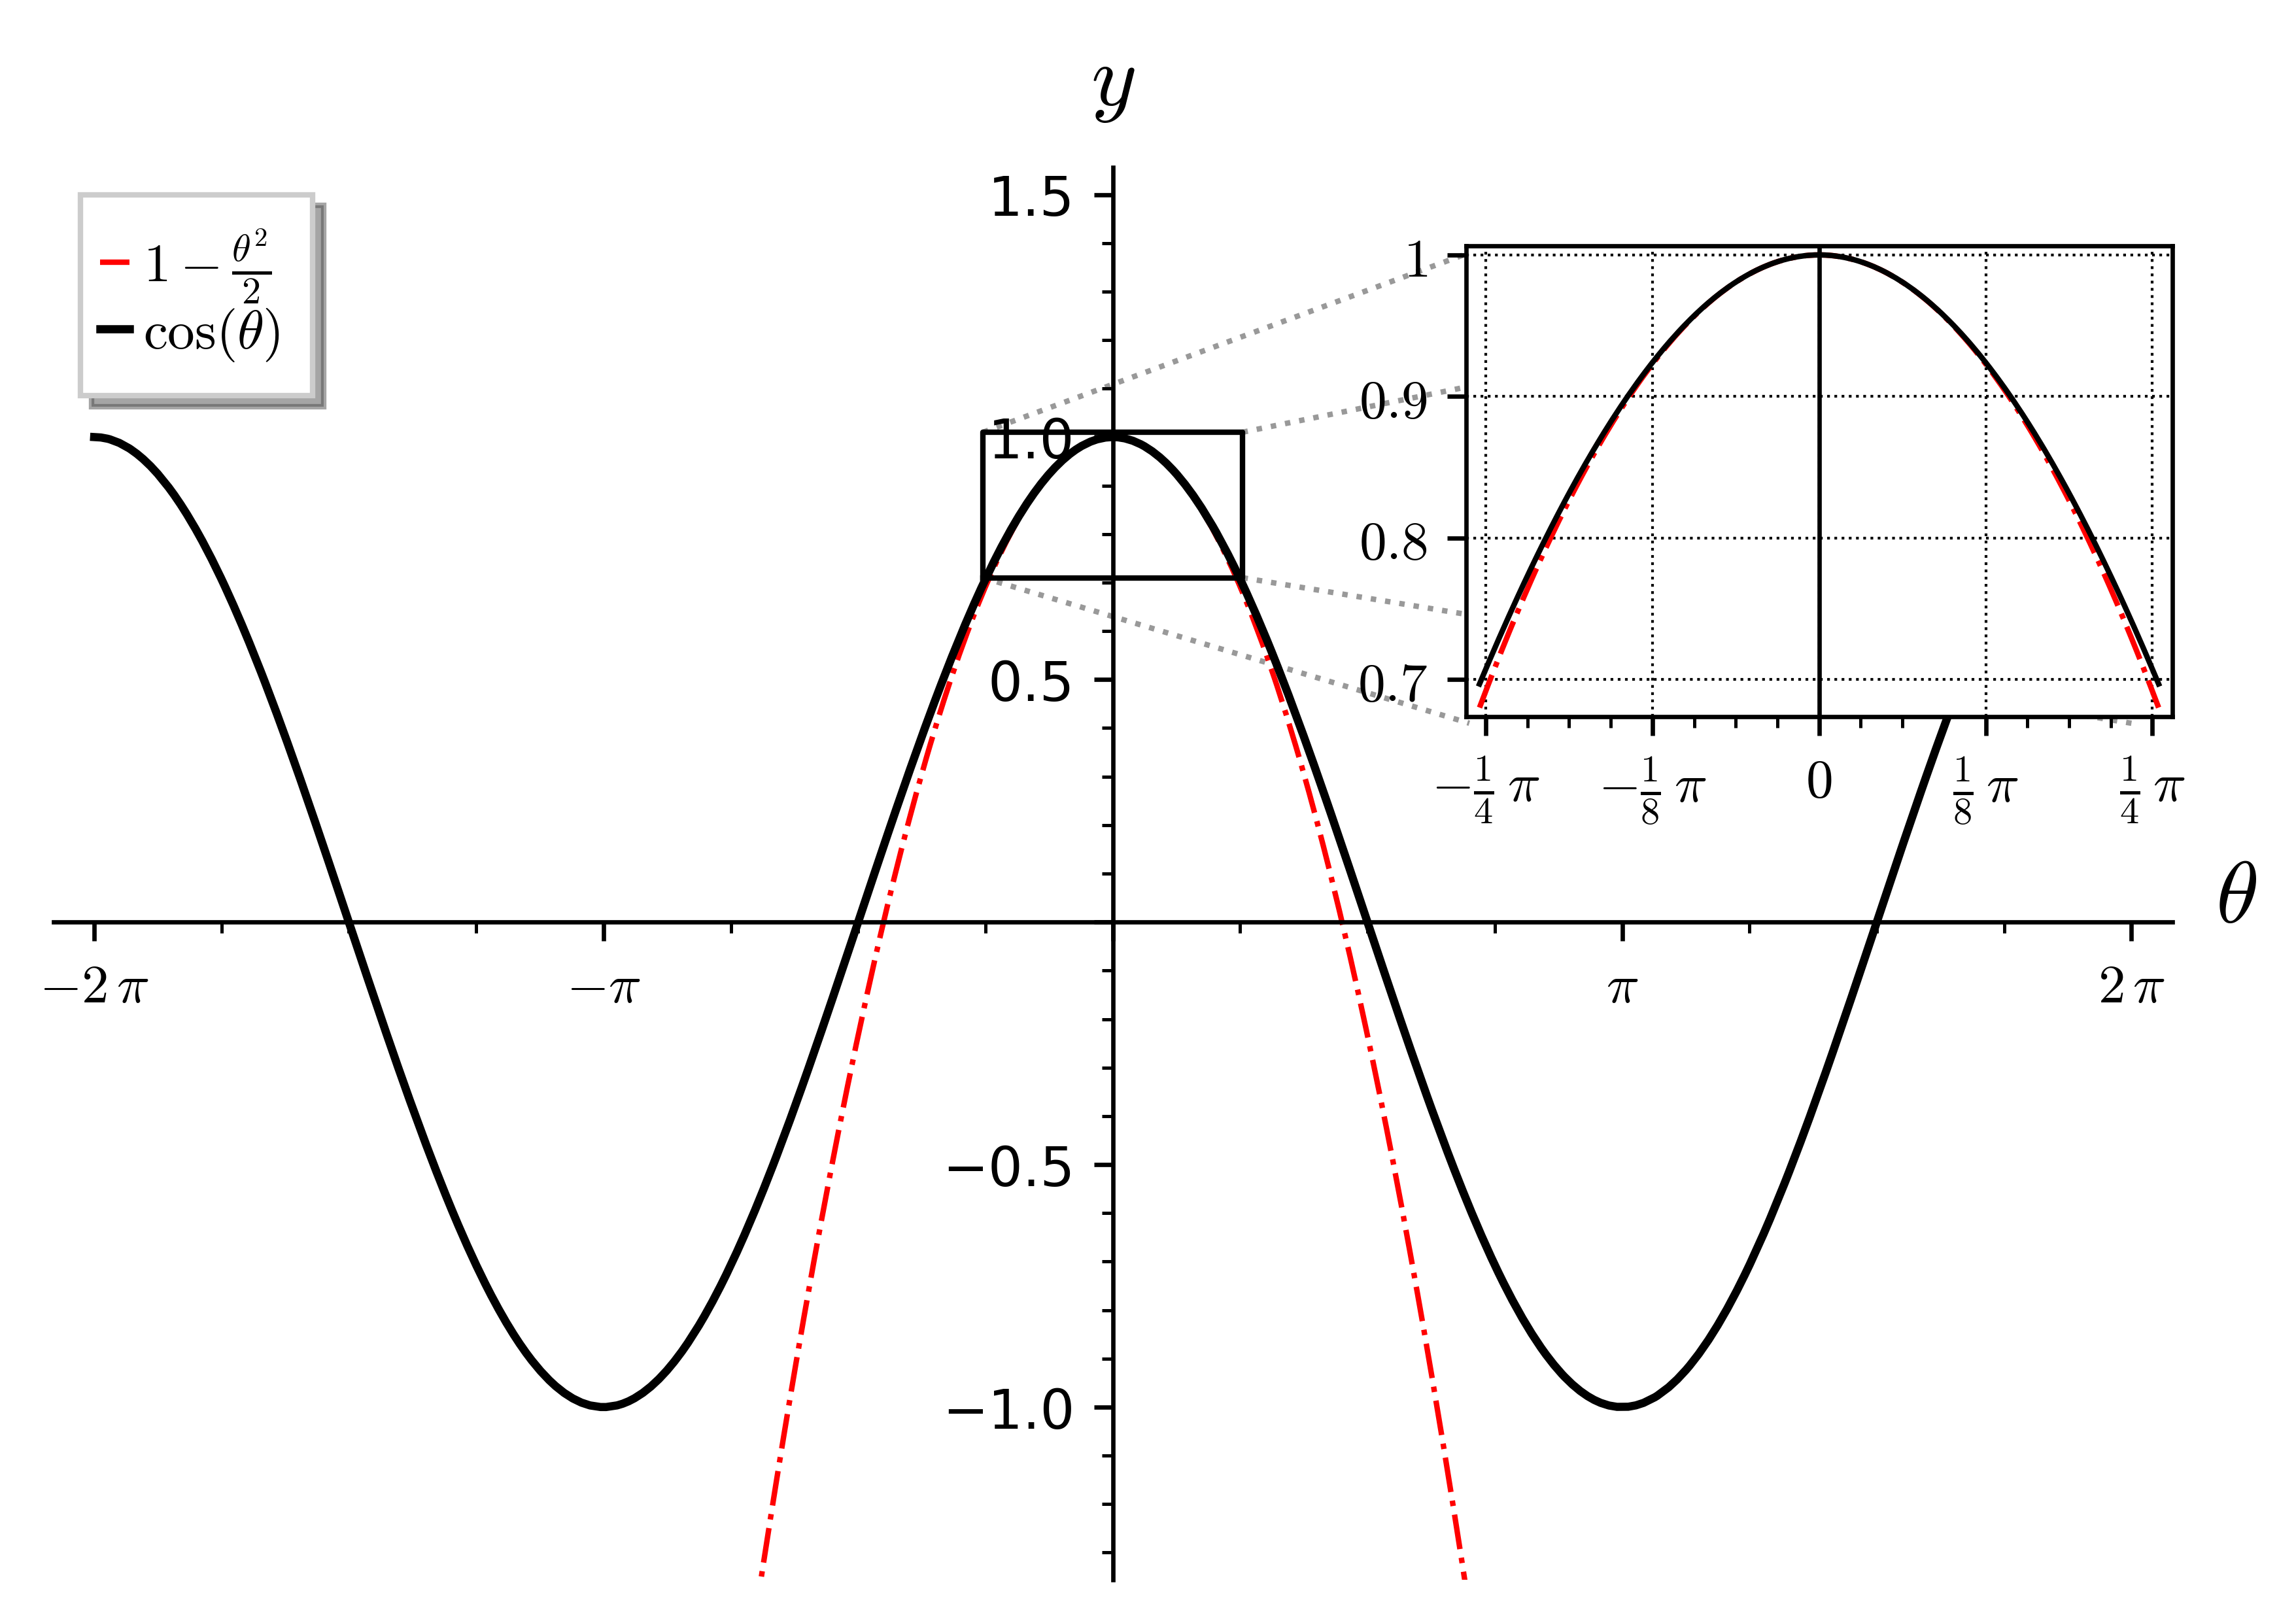
\includegraphics[width=\textwidth]{figures/cosinuszoom.png}
     \caption{Andengradstaylorpolynomium for $\cos(\theta)$}
     \label{fig:cosinusanden}
\end{figure}\\
Det er tydeligt på Figur \ref{fig:cosinusanden}. at denne approksimation er god for små værdier af $\theta$. Lad os undersøge hvor korrekt den er på $\theta=\frac{1}{8}\pi$
\begin{equation*}
    P_2\left(\frac{\pi}{8}\right)=0{,}9228937
\end{equation*}
\[
n=2, a=0, x=\frac{\pi}{8}, \quad a<\xi<x
.\] 
Vi kan benytte os af Taylors formel med restled, hvor $n=2$, fordi det er et andengradstaylorpolynomium.  $a=0$, fordi vores udviklingspunkt er 0,  $x=\frac{\pi}{8}$, fordi det er punktet som vi approksimerer, og ifølge Lagrangeformen for restled skal $\xi$ ligge i intervallet $]a;x[$:
\begin{equation*}
    \begin{aligned}
    f(x)&=f(a)+f'(a)(x-a)+\frac{f''(a)}{2!}(x-a)^2+\frac{f'''(\xi)}{3!}(x-a)^3\\
    f\left(\frac{\pi}{8}\right)&=f(0)+f'(0)(x-0)+\frac{f''(0)}{2!}(x-0)^2+\frac{f'''(\xi)}{3!}(x-0)^3\\
    f\left(\frac{\pi}{8}\right)&=f(0)+f'(0)\left(\frac{\pi}{8}\right)+\frac{f''(0)}{2!}\left(\frac{\pi}{8}\right)^2+\frac{f'''(\xi)}{3!}\left(\frac{\pi}{8}\right)^3\\
    f\left(\frac{\pi}{8}\right)&=1-\frac{1}{2!}\left(\frac{\pi}{8}\right)^2+\frac{\sin(\xi)}{3!}\left(\frac{\pi}{8}\right)^3\\
    f\left(\frac{\pi}{8}\right)&=1-\frac{\pi^2}{128}+\frac{\sin(\xi)\pi^3}{3072}\\
%        \cos\left(\frac{\pi}{8}\right)&\approx 0{,}9228937 - \frac{f'''(\xi)}{3!}(x-a)^3\\
%                                       &\approx 0{,}9228937 - \frac{\sin(\xi)}{6}(x-a)^3\\
    \end{aligned}
\end{equation*}
Vi har nu forsiimplet denne ligning, og vi kan bruge dette til at finde den maksimale fejl af approksimationen.\\
Dette finder vi ved at undersøge hvornår $R_2\left(\frac{\pi}{8}\right)=\frac{\sin(\xi)\pi^3}{3072}$ indtager den største værdi. Det er nemt at se, fordi $\sin(\xi)$ ligger i tælleren, og vi ved at  $(0<\xi<\frac{\pi}{8})$.\\
Restleddet kan derfor ikke være større end når $\xi=\frac{\pi}{8}$. Dette indsætter vi i restleddet.
\begin{equation*}
    \frac{\sin\left(\frac{\pi}{8}\right)\pi^3}{3072}\approx 0{,}00386
\end{equation*}
Vi ved altså med sikkerhed at vores approksimation er rigtig med 2 decimaler.\\
For at finde den nøjagtige fejl finder vi blot differencen mellem $P_2(x)$ og $f(x)$ :
\begin{equation*}
    \left|P_2\left(\frac{\pi}{8}\right)-f\left(\frac{\pi}{8}\right)\right|=\left|1-\frac{\pi^2}{128}-\cos\left(\frac{\pi}{8} \right)   \right|\approx 0{,}00098582
\end{equation*}
Vi kan se, at vores maksimale fejl er større end den faktiske fejl, hvilket er som forventet.
\section{Praktiske anvendelser af Taylorpolynomier}
I den digitale tidsalders barndom troede man i en periode, at Taylorpolynomier hovedsageligt ville have historisk interresse, men det har vist sig, at kendskab til disse metoder stadig i dag er relevant. Når man sender robotter til Mars, eller undersøger fysiske fenomener på nano-niveau, kræver det kompliceret og præcis matematik, hvor Taylorpolynomier ofte finder sin plads.\footcite[s. 11]{hvadermatematik}\\
Det er dog ikke kun studiet af fjerne planeter og små atomer der drager udbytte af denne regnemetode. Taylorpolynomier er også en del af den teori, der danner grund for mange af de elektroniske apparater, som vi bruger hver dag. 
\subsection{I computervidenskab}
Taylorpolynomier kan have meget fundamentale anvendelser. Man kan forestille sig en computer der kun kan addere $(+)$, subtrahere $(-)$ og multipicere $(\times)$, men ikke dividere $(\div)$. Ville sådan en computer kunne udregne en brøk?\\
I dette scenarie kunne man bruge et enkelt Taylorpolynomium. Nemlig Taylorpolynomiet for en geometrisk serie:
\begin{equation*}
    \begin{aligned}
        \frac{1}{1-x}&\approx 1+x+x^2+x^3+\cdots+x^n, \quad |x|<1\\
    \end{aligned}
\end{equation*}
Vi kan fx. approksimere $\sfrac{329}{73}$ med denne metode, helt uden at dividere:\footcite[s. 646]{calculuswithanalyticgeometry}\\
\begin{equation*}
    \begin{aligned}
        \frac{329}{73}&=\frac{3{,}29}{0{,}73}=3{,}29\cdot\frac{1}{1-0{,}27}\\
                      &\approx 3{,}29\cdot\left(1+0{,}27+0{,}27^2+\cdots+0{,}27^{10}\right)\\
                      &\approx3{,}29\cdot1{,}36986\\
        \frac{329}{73}&\approx 4{,}5068
    \end{aligned}
\end{equation*}
I virkeligheden bruger computere dog ikke denne metode. De bruger hurtigere algoritmer så som Goldschmidts eller Newton-Raphsons algoritmer.\footcite{division}, men der er andre problemer der konkret løses med viden, som den der findes i Taylorpolynomier, eksempelvis integralet af \textit{transcendente} funktioner så som $\sin(x), \cos(x), e^x \text{ og } \ln(x)$. Computere drager isér ofte nytte af Taylorpolynomier når de for eksempel i videospil skal udregne trigonometriske funktioner hurtigt og effektivt.\footcite[11]{hvadermatematik}
\subsection{I økonomi}
Matematikken i økonomi kan også blive svær at have med at gøre, og også her finder Taylorpolynomier andvendelse. et eksempel på dette er \textit{Black-Scholes} formlen, der kan bruges til at udregne prisen for en option på en aktie, hvor Taylorpolynomier tit bruges i formlens implementering, men her er det vigtigt at have indgående kendskab til Taylorpolynomier, for ikke at bruge dem forkert. \footcite{aktier}
\subsection{I fysik}
Differentialligninger kan være meget svære at have med at gøre, men Taylorpolynomer gør dem nemme. Dette er nyttigt i mange områder af fysik, det kan være når man studerer elektriske felter, når man optimerer fysiske systemer for at studere et equilibrium i en klump atomer, studiet af porøse stenarters elasticitet eller når man man modellerer havbølgers færden over ujævnt terræn\footcite{applicationsoftaylor}\\
\\
Taylorpolynomier er altså et fundamentalt matematisk værktøj, og deres anvendelser kan brede sig ud over stort set alle fag, hvor matematik er involveret. Desuden danner de basis for mange af de digitale reccourcer, som vi tager for givet i vores daglige brug af elektroniske værktøjer.

\section{Konklusion} % samle problemformuleringens underspørgsmål. "jeg har. og så... jeg kan konkludere..."
\newpage
\section{Litteraturliste}
\subsection{Referenceliste}
\printbibliography[title=Cited]
\end{refsection}
\subsection{Litteraturliste}
\nocite{*}
\printbibliography
%\printbibliography[keyword=online]
Forsidebillede samt alle figurer er skabt af undertegnede.
\end{document}

